\documentclass[10pt]{beamer}

\usepackage{fontspec}

%% Minted setup (syntax highlighting)
\usepackage[outputdir=latex.out]{minted}
\usemintedstyle{vs}
\setminted{fontsize=\footnotesize}
\newminted[code]{scala}{gobble=0, escapeinside=@@}
\newenvironment{slide}[2][]
  {\begin{frame}[fragile,environment=slide,#1]{#2}}
  {\end{frame}}
\newcommand\makemintedshortinline[2]{%
  \catcode`#2=13
  \begingroup%
  \lccode`\~=`#2
  \lowercase{\endgroup\protected\def~{\mintinline[escapeinside=@@]{#1}~}}%
}
\renewcommand{\fcolorbox}[4][]{#4}

%% Beamer theme setup
\usetheme[block=fill]{metropolis}
\setbeamercolor{progress bar}{bg=black, fg=black}
\setbeamercolor{title separator}{bg=black, fg=black}
\setbeamercolor{progress bar in head/foot}{bg=black, fg=black}
\setbeamercolor{progress bar in section page}{bg=black, fg=black}
\setbeamercovered{transparent}

\usepackage{xspace}
\usepackage{mathtools}
\def\A{\normalfont\text{A}}
\def\B{\normalfont\text{B}}
\def\C{\normalfont\text{C}}
\def\D{\normalfont\text{D}}
\def\T{\normalfont\text{T}}
\def\<:{\allowbreak\operatorname{\normalfont\text{<}:}\allowbreak}
\def\Fsub{\normalfont{F}\ensuremath{_{\<:}}\xspace}

\usepackage[autostyle=false, style=english]{csquotes}
\MakeOuterQuote{"}

\usepackage{xcolor}
\definecolor{typeColor}{HTML}{2B91B0}
\definecolor{implColor}{HTML}{57B5E8}
\definecolor{singColor}{HTML}{009E73}
\definecolor{mtpeColor}{HTML}{9400D4}
\newcommand{\tp}[1]{\color{typeColor}#1}

\usepackage{tikz}
\usetikzlibrary{decorations.pathreplacing,positioning, arrows.meta}

\title{Abstractions for Type-Level Programming}
\date{Tuesday, 22 March 2022}
\author{Olivier Blanvillain}

\makemintedshortinline{scala}\|

\newcommand{\timeline}[5] {
  \begin{tikzpicture}
    \draw[lightgray!#5!black, thick, -Triangle] (0,0) -- (10cm,0);
    \foreach \x in {0,1,...,6}
    \draw[lightgray!#5!black] (\x*1.4 cm,3pt) -- (\x*1.4 cm,-3pt);

    \foreach \x/\descr in {0/2016,1/2017,2/2018,3/2019,4/2020,5/2021,6/2022}
    \node[lightgray!#5!black, font=\scriptsize, text height=1.75ex,
    text depth=.5ex] at (\x*1.4,-.3) {$\descr$};

    \fill[lightgray!#1!implColor] (0.25, 0.5) circle (4pt) node[lightgray!#1!black,align=center,above=7pt,font=\small]{DataFrame\\Library};

    \draw[lightgray!#2!singColor, line width=4pt]
    (2.25*1.4,.5) -- (4.417*1.4,.5) node[lightgray!#2!black,midway,above=5pt,font=\small]{Generalized Singletons};

    \draw[lightgray!#3!mtpeColor, line width=4pt]
    (2.5*1.4,-.7) -- (6.15*1.4,-.7) node[lightgray!#3!black,midway,below=5pt,font=\small]{Match Types};
    \draw[thick,lightgray!#3!mtpeColor,-Triangle,line width=1.2pt] (6.15*1.4,-.7) -- (6.25*1.4,-.7);

    \fill[lightgray!#4!mtpeColor] (6.1*1.4, 0.5) circle (4pt) node[lightgray!#4!black,align=center,above=7pt,font=\small]{Regex\\Library};
  \end{tikzpicture}
}
% Jun 12 2018  Add TypeOf  #4671
% Sep 20 2018  Add match type #4964
% ECOOP  Jan 12 → Apr 1  2019, rejected
% OOPSLA Mai 15 → Aug 1  2020, rejected
% PLDI   Nov 20 → Feb 25 2021, rejected
% OOPSLA Apr 16 → Jul 2  2021, rejected
% POPL   Jul 7  → Sep 28 2021, accepted

\begin{document}

\maketitle

\begin{slide}{Example 1: Database queries (2016)}
\begin{center}

\includegraphics[width=0.3\textwidth]{figures/spark.pdf}
\end{center}
\end{slide}

\begin{slide}{Example 1: Database queries (2016)}
Spark APIs are practically untyped:
\begin{code}
class DataFrame {
  /** Inner equi-join with another DataFrame on the given column.
   *  The join column will only appear once in the output. */
  def join(right: DataFrame, column: String): DataFrame
}
\end{code}
\pause
Revisited with type-level programming:
\begin{code}
class DF[X] {
  def join[Y](df: DF[Y], col: String): DF[col+(X-col)++(Y-col)]
}
\end{code}
\end{slide}

\begin{slide}{Example 2: Regular expressions (2022)}
Regular expressions in Scala's standard library:
\begin{code}
val rational = new Regex("(\\d+)\\.?(\\d+)?")
rational.unapply("3.1415"): Option[Seq[String]]
\end{code}
\pause
Revisited with type-level programming:
\begin{code}
rational.unapply("3.1415"): Option[(String, Option[String])]
\end{code}
\pause
\begin{code}
class Regex(pattern: String) {
  def unapply(s: String): Option[GroupsOf[@pattern@]]
}
\end{code}
\end{slide}

\begin{slide}{What changed between 2016 and 2022?}
\begin{tikzpicture}
  \draw[black, thick, -Triangle] (0,0) -- (10cm,0);
  \foreach \x in {0,1,...,6}
  \draw[black] (\x*1.4 cm,3pt) -- (\x*1.4 cm,-3pt);

  \foreach \x/\descr in {0/2016,1/2017,2/2018,3/2019,4/2020,5/2021,6/2022}
  \node[black, font=\scriptsize, text height=1.75ex,
  text depth=.5ex] at (\x*1.4,-.3) {$\descr$};

  \fill[implColor] (0.25, 0.5) circle (4pt) node[black,align=center,above=7pt,font=\small]{DataFrame\\Library};

  \fill[mtpeColor] (6.1*1.4, 0.5) circle (4pt) node[black,align=center,above=7pt,font=\small]{Regex\\Library};
\end{tikzpicture}
\end{slide}

\begin{slide}{What changed between 2016 and 2022?}
Example 1 uses a hack, implicits:
\begin{itemize}
  \item convoluted to use
  \item slow to compile
\end{itemize}

Example 2 uses a new language construct, match types, one of the main contributions of this thesis.
\end{slide}

\begin{slide}{Compilation times for the type-level join operation}
\begin{center}
\input{figures/join.gex}
\end{center}
\end{slide}

\begin{slide}{Timeline of my PhD}
\timeline{0}{0}{0}{0}{0}
\end{slide}

\begin{slide}{Part I: Generalized Singleton Types}
\timeline{80}{0}{80}{80}{80}
\end{slide}

\begin{slide}{Singleton types}
Scala supports a few singleton types:
\begin{itemize}
  \item |x.type|, the type of the variable |x| (since forever)
  \item |42|, the type of the integer literal |42| (since 2016)
  \item |+|, the type of integer addition (since 2020)
\end{itemize}
\pause
Question: How much of the language can we represent in types?
\end{slide}

\begin{slide}{Generalized singleton types: A proposal}
Our proposal consists of 3 changes:
\begin{enumerate}
  \item new types for if-then-else, pattern matching, constructors, functions calls
  \item "precise mode" of type inference
  \item type evaluation, during subtyping
\end{enumerate}
\end{slide}

\begin{slide}{New types}
What's the type of | if (x == 0) "zero" else "one"|?
\begin{itemize}
  \pause\item |String| ~(Scala 2)
  \pause\item |"zero"|~{\footnotesize\texttt\textbar}~|"one"| ~(Scala 3)
  \pause\item |If[x.type == 0,|| "zero", "one"]| ~(proposed)
  \pause\item |{ if (x == 0) "zero" else "one" }| ~(proposed, syntactic sugar)
\end{itemize}
\pause
Similarly, we add new types for other constructs: |Match[]|, |New[]| and |Call[]|, and the corresponding syntactic sugar.
\end{slide}

\begin{slide}{"Precise mode" of type inference}
We need two modes of type inference, for backwards compatibility.

\vspace{5pt}
\begin{overprint}
\onslide<1>
\begin{code}
@\phantom{dependent}@
def int2str(x: Int) =
  if (x == 0) "zero" else "one"
\end{code}

\onslide<2>
\begin{code}
@\phantom{dependent}@
def int2str(x: Int): String =
  if (x == 0) "zero" else "one"
\end{code}

\onslide<3>
\begin{code}
dependent
def int2str(x: Int)
  : { if (x @\tp{== 0}@) "zero" @\tp{else}@ "one" }
  =   if (x == 0) "zero" else "one"
\end{code}

\onslide<4-5>
\begin{code}
dependent
def int2str(x: Int)
  : If[x.type @\tp{== 0}@, "zero", "one"]
  =   if (x == 0) "zero" else "one"
\end{code}

\onslide<6>
\begin{code}
dependent
def int2str(x: Int)
  : If[x.type @\tp{== 0}@, "zero", String]
  =   if (x == 0) "zero" else readString()
\end{code}

\onslide<7>
\begin{code}
dependent
def int2str(x: Int)
  : { if (x @\tp{== 0}@) "zero" @\tp{else}@ (_: String) }
  =   if (x == 0) "zero" else readString()
\end{code}
\end{overprint}
\medskip
\pause\pause\pause\pause

The "precise mode" is best effort: it lifts whatever possible to the type level and approximates the rest.
\end{slide}

\begin{slide}{"Precise mode" of type inference: list concatenation example}
\begin{code}
dependent def concat(xs: List, ys: List) <: List =
  xs match
    case x :: xs => x :: concat(xs, ys)
    case Nil => ys
\end{code}
\pause
\begin{overprint}
\onslide<1-2>
\begin{code}
dependent val l1 = "A" :: Nil
dependent val l2 = "B" :: Nil
dependent val l3 = concat(l1, l2)
l3: { "A" :: "B" :: Nil }
\end{code}

\onslide<3>
\begin{code}
val l1: List     = "A" :: Nil
dependent val l2 = "B" :: Nil
dependent val l3 = concat(l1, l2)
l3: { concat(l1, l2) }
\end{code}

\onslide<4>
\begin{code}
dependent val l1 = "A" :: Nil
val l2: List     = "B" :: Nil
dependent val l3 = concat(l1, l2)
l3: { "A" :: l2 }
\end{code}

\end{overprint}
\end{slide}

\begin{slide}{Type evaluation}
During subtyping, we evaluate both sides:
\begin{code}
A <: B  iff  eval(A) <: eval(B)
\end{code}
\pause

Straightforward for if-then-else:
\begin{code}
eval(If[true, A, B]) = A
eval(If[false, A, B]) = B
\end{code}
\pause

More interesting for pattern matching: we "desugar" pattern matching expressions into if-then-else \& type tests.
\pause
\smallskip

We evaluate type tests using subtyping and type disjointness:
\begin{code}
eval(@\tp{x.asInstanceOf}@[Foo]) = true   iff  x.type <: Foo
eval(@\tp{x.asInstanceOf}@[Foo]) = false  iff  disj(x.type, Foo)
\end{code}
\end{slide}

\begin{slide}{Type evaluation: pattern matching example}
\begin{overprint}
\onslide<1>
\begin{code}
dependent val foo(x: Any) =
  x match
    case s: String => s
    case i: Int => i+1
\end{code}
\onslide<2>
\begin{code}
dependent val foo(x: Any): {
  x match
    case s: String => @\tp{s}@
    @\tp{case i: Int}@ => @\tp{i+1}@
} =
  x match
    case s: String => s
    case i: Int => i+1
\end{code}
\onslide<3->
\begin{code}
dependent val foo(x: Any): {
  if (x.isInstanceOf[String]) x.asInstanceOf[String]
  @\tp{else if }@(@\tp{x.isInstanceOf}@[@\tp{Int}@]) @\tp{x.asInstanceOf}@[Int] @\tp{+ 1}@
  @\tp{else throw new}@ MatchError()
} =
  x match
    case s: String => s
    case i: Int => i+1
\end{code}
\end{overprint}
\bigskip

\begin{overprint}
\onslide<4>
|foo(42): { foo(42) }|
\onslide<5>
|foo(42): { 42.asInstanceOf[Int] + 1 }|
\onslide<6>
|foo(42): { 42 + 1 }|
\onslide<7>
|foo(42): { 43 }|
\onslide<8->
|foo(42): 43|
\end{overprint}

\begin{overprint}
\onslide<9>
|foo(readString())|
\onslide<10>
|foo(readString()): { foo(_: String) }|
\onslide<11>
|foo(readString()): { (_: String).asInstanceOf[String] }|
\onslide<12>
|foo(readString()): { (_: String) }|
\onslide<13>
|foo(readString()): String|
\end{overprint}
\end{slide}

\begin{slide}{Generalized Singletons: Recap}

We proposed the following 3 changes:
\begin{enumerate}
  \item lift a subset of Scala's language constructs to the type level
  \item add a "precise mode" of type inference
  \item evaluate those types during subtyping
\end{enumerate}
\end{slide}

% Termination
% Virtual dispatch

\begin{slide}{Part II: Match Types}
\timeline{80}{80}{0}{80}{80}
\end{slide}

\begin{slide}{Overview}
\begin{code}
type Elem[X] = X match
  case String => Char
  case List[t] => Elem[t]
  case Any => X
\end{code}
\end{slide}

\begin{slide}{Disjointness}
|Elem[Seq[Int]]| is stuck
\end{slide}

\begin{slide}{Relating match terms and types: a defining property}
|Elem[Seq[Int]]| is stuck
\end{slide}

\begin{slide}{Formalizing Match Types}
System FM is an extension of System \Fsub with
\begin{itemize}
  \item pattern matching
  \item opaque classes
  \item match types
\end{itemize}
Design goals:
\begin{itemize}
  \item explain the essence of match types
  \item give us confidence in our design
  \item be as simple as possible
\end{itemize}
\end{slide}

\begin{slide}{System FM is parametric}
System FM is parametrized by a set of externally defined classes:

FM(C, $\Psi$, $\Xi$)
\begin{itemize}
  \item $\C \hspace{2.3pt} \coloneqq$ set of classes
  \item $\Psi \coloneqq$ class inheritance relation
  \item $\Xi \hspace{1.1pt} \coloneqq$ class disjointness relation
\end{itemize}
\pause
For example:

\begin{tabular}{@{}llll@{}}
|class A|          &$\C = \{\A\}$     & $\Psi = \varnothing$  & $\Xi = \varnothing$\\
|class A; class B extends @\tp{A}@| &$\C = \{\A, \B\}$ & $\Psi = \{(\B, \A)\}$ & $\Xi = \varnothing$\\
|class A; class D| &$\C = \{\A, \D\}$ & $\Psi = \varnothing$  & $\Xi = \{(\A, \D)\}$\\
|class A; trait T| &$\C = \{\A, \T\}$ & $\Psi = \varnothing$  & $\Xi = \varnothing$\\
\end{tabular}
\end{slide}

\begin{slide}{System FM's syntax}
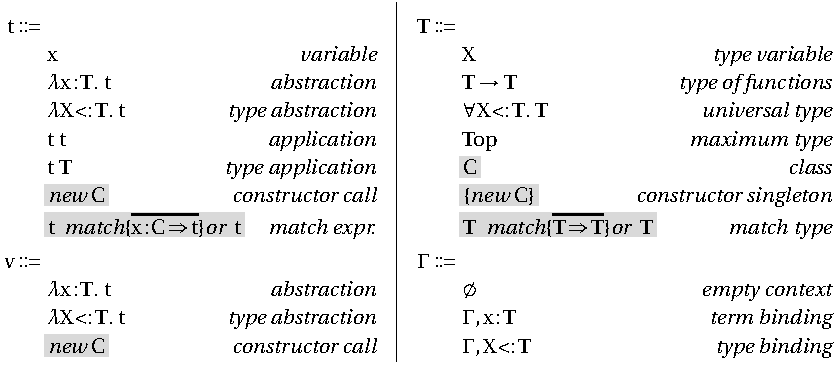
\includegraphics[width=\textwidth]{figures/FMSyntax.pdf}
\end{slide}

\begin{slide}{System FM's pattern matching evaluation}
Given a concrete scrutinee, we evaluate match expressions with a few lookups in the inheritance relation:
\begin{center}
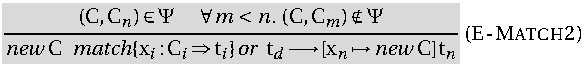
\includegraphics[width=0.8\textwidth]{figures/FMEMatch.pdf}
\end{center}
\end{slide}

\begin{slide}{System FM's disjointness relation}
\begin{center}
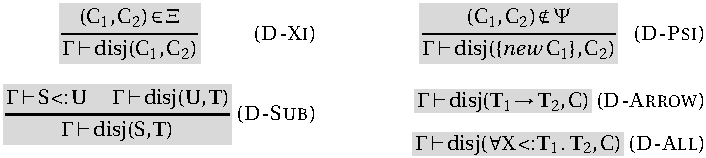
\includegraphics[width=0.9\textwidth]{figures/FMDisjointness.pdf}
\end{center}
\end{slide}

\begin{slide}{System FM's match types evaluation rule (subtyping)}
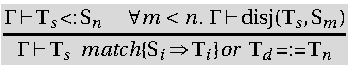
\includegraphics[width=\textwidth]{figures/FMSMatch.pdf}
\end{slide}


\begin{slide}{System FM's type safety}
We show type safety through the progress and preservation.

Our proof comes in two versions:
\begin{enumerate}
  \item Pen and paper (\textasciitilde30 pages)
  \item Coq mechanization (\textasciitilde6000 LOC)
\end{enumerate}
\end{slide}

\begin{slide}{Structure of the type safety proof}
\begin{center}
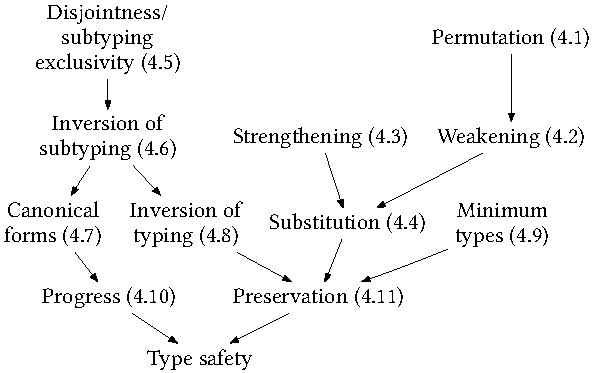
\includegraphics[width=0.8\textwidth]{figures/FMProofStructure.pdf}
\end{center}
\end{slide}

\begin{slide}{Empty Types}
Our system does not like empty types.

|Nothing|, in particular, is both subtype and disjoint from every type.

Intersections require special care.

\pause

\begin{code}
type M[X] = X match
  case Int => String
  case String => Int

class C:
  type X
  def f(bad: M[X & String]): Int = bad

class D extends C:
  type X = Int
\end{code}
\end{slide}

\begin{slide}{Variance}
At first glance, we can't prove disjointness when variance is involved.

|F[+T]:| \quad |T1 <: T2| \quad implies \quad |F[T1] <: F[T2]|\\
|G[-T]:| \quad |T1 <: T2| \quad implies \quad |G[T1] >: G[T2]|
\pause

We make an exception for covariant type that are used as class fields:
\begin{code}
case class Some[+A](value: A)
\end{code}

|Some[String]| and |Some[Int]| are disjoint, since there is no runtime value of type |Some[Nothing]|.

\end{slide}

\begin{slide}{Match Types, Conclusion}
TODO
\end{slide}

\begin{slide}{Thank you!}
\timeline{0}{0}{0}{0}{0}
\end{slide}

\appendix

\begin{slide}{Type-Safe Regular Expressions (simplified)}
\begin{code}
val rational = new Regex("(\\d+)\\.(\\d+)")
rational.unapply("3.1415"): Option[(String, String)]

type GroupsOf[P <: String] =
  Reverse[Loop[P, 0, Length[P], EmptyTuple]]

type Loop[P, Lo, Hi, Acc <: Tuple] =
  Lo match
    case Hi => Acc
    case _ => CharAt[P, Lo] match
      case '('  => Loop[P, Lo + 1, Hi, String *: Acc]
      case '\\' => Loop[P, Lo + 2, Hi, Acc]
      case _ => Loop[P, Lo + 1, Hi, Acc]
\end{code}
\end{slide}

% \appendix
\end{document}
